\subsection{Context Closure}
It is crucial to ensure that the weight of any object subject to rewriting is greater than or equal to $1_\mathcal{S}$.
% not $0_S$, because \(0_S\) behaves unpredictably in well-founded semirings. For instance, in the natural and real tropical semirings \((\mathbb{N} \cup \{+\infty\}, \min, +, +\infty, 0_S, <, \leq)\), \(0_S\) is the greatest element \(+\infty\), while in the natural and real arctic semirings \((\mathbb{N} \cup \{-\infty\}, \max, +, -\infty, 0_S, <, \leq)\), \(0_S\) is the smallest element \(-\infty\).
This issue is addressed by the existence of a context closure. Specifically, it ensures that every graph that can be rewritten using that rule admits some morphism into the weighted type graph, and thus the weight of the morphism, which is the sum of the weights of the morphisms into the type graph, is greater than or equal to \(1_S\) by \autoref{lem:wf:morphism_weight_geq_1_neq_0}.
\label{sec:context_closure}
% \begin{remark} 
%   \label{remark:semiring_0_unpredictable}
%   The requirement \textquote{for all \(e \in \mathbb{E}, w(e) \neq 0_S\)} is necessary because \(0_S\) behaves unpredictably in strongly monotonic measurable semirings. For instance, in the natural and real tropical semirings \((\mathbb{N} \cup \{+\infty\}, \min, +)\), \(0_S\) is the greatest element \(+\infty\), while in the natural and real arctic semirings \((\mathbb{N} \cup \{-\infty\}, \max, +)\), \(0_S\) is the smallest element \(-\infty\).
% \end{remark} 

\begin{definition}[Context Closure~\cite{endrullis2024generalized_arxiv_v2}]
    \label{def:context_closure}  
    \ \newline 
\begin{minipage}{0.65\textwidth}
    Let $\mathcal{T}=(T,\mathbb{E},\mathcal{S},w)$ be a finitary weighted type graph, \(\rho = (L \overset{l}{\leftarrow} K \overset{r}{\rightarrow} R ) \) a DPO rewriting rule and $\mathfrak{F}$ a rewriting framework. 
    A \textbf{context closure} for $\rho$ and $\mathcal{T}$ in $\mathfrak{F}$ is a morphism $c:L \rightarrow T$ such that for every DPO diagram in $\mathfrak{F}(\rho)$ (shown on the right) 
    there exists $\alpha : G \rightarrow T$ such that $m \star \alpha = c$.
\end{minipage}
\begin{minipage}{0.35\textwidth}
    \begin{center}
        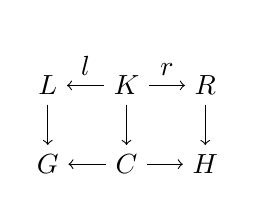
\begin{tikzpicture}[node distance=11mm]
          \node (I) at (0,0) {$K$};
          \node (L) at (-1,0) {$L$};
          \node (R) at (1,0) {$R$};
          \node (G) at (-1,-1) {$G$};
          \node (C) at (0,-1) {$C$};
          \node (H) at (1,-1) {$H$};
          \draw [->] (I) to node [label, above] {$l$} (L);
          \draw [->] (I) to node [label,above] {$r$} (R);
        %   \draw [->] (L) to node [label, right] {$m$} (G);
        \draw [->] (L) to node [label, right] {} (G);
          \draw [->] (I) to (C);
          \draw [->] (R) to (H);
          \draw [->] (C) to (G);
          \draw [->] (C) to (H);
        \end{tikzpicture}
      \end{center}
\end{minipage}
\end{definition}
\begin{example}
    \label{wf:example:context_closure}
    Let the set of edge labels be $\Sigma = \{a,b\}$.
    Consider the DPO rule in~\autoref{ex:nwf:grsaa_rule}.
    \begin{figure}[!ht]
     \centering 
      \resizebox{0.7\textwidth}{!}{
      \begin{tikzpicture}
          \graphbox{$L$}{0mm}{0mm}{34mm}{15mm}{2mm}{-5mm}{
              \coordinate (o) at (0mm,-3mm); 
              \node[draw,circle] (l1) at ($(o)+(-10mm,0mm)$) {1};
              \node[draw,circle] (l2) at ($(l1)+(2,0)$) {2};
              \node[draw,circle] (l3) at ($(l1) + (1,0)$) {3};
              \draw[->] (l1) -- (l3) node[midway,above] {a};
              \draw[->] (l3) -- (l2) node[midway,above] {a};
          }     
          \graphbox{$K$}{40mm}{0mm}{24mm}{15mm}{2mm}{-5mm}{
              \coordinate (o) at (5mm,-3mm); 
              \node[draw,circle] (l1) at ($(o)+(-10mm,0mm)$) {1};
              \node[draw,circle] (l2) at ($(l1)+(1,0)$) {2};
              % \node[draw,circle] (l3) at ($(l1) + (1,0)$) {$\ $};
              % \draw[->] (l1) -- (l3) node[midway,above] {a};
              % \draw[->] (l3) -- (l2) node[midway,above] {a};
          }    
          \graphbox{$R$}{70mm}{0mm}{45mm}{15mm}{2mm}{-5mm}{
              \coordinate (o) at (-5mm,-3mm); 
              \node[draw,circle] (l1) at ($(o)+(-10mm,0mm)$) {1};
              \node[draw,circle] (l2) at ($(l1)+(3,0)$) {2};
              \node[draw,circle] (l3) at ($(l1) + (1,0)$) {4};
              \node[draw,circle] (l4) at ($(l1) + (2,0)$) {5};
              \draw[->] (l1) -- (l3) node[midway,above] {a};
              \draw[->] (l3) -- (l4) node[midway,above] {b};
              \draw[->] (l4) -- (l2) node[midway,above] {a};
          }    
          \node () at (37mm,-8mm) {$\overset{l}{\leftarrowtail}$};
          \node () at (67mm,-8mm) {$\overset{r}{\rightarrowtail}$};
          % \draw[>->] (51mm,2mm) -- (52mm,3mm);
      \end{tikzpicture}
      }
      \caption{}
      \label{ex:nwf:grsaa_rule}
  \end{figure}
   and the weighted type graph in \autoref{fig:nwf:weighted_type_graph_grsaa} shown below
  \begin{figure}[!ht]
        \centering
        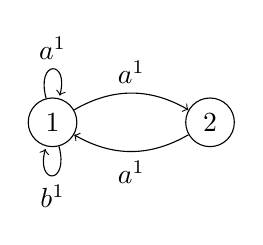
\begin{tikzpicture}
            \graphbox{}{0mm}{0mm}{32mm}{28mm}{-10mm}{-14mm}{
                \node[draw,circle] (1) at (0,0) {1};
                \node[draw,circle] (2) at (2,0) {2};
                \draw[->] (1) edge[loop above] node[midway, above] {$a^{1}$} (1) ;
                \draw[->] (1) edge[loop below] node[midway, below] {$b^{1}$} (1) ;
                \draw[->] (1) edge[bend left] node[midway, above] {$a^{1}$}  (2)  ;
                \draw[->] (2) edge[bend left] node[midway, below] {$a^{1}$} (1)   ;
            }
        \end{tikzpicture}
        \caption{}
        \label{fig:nwf:weighted_type_graph_grsaa}
    \end{figure}
   Let $c$ be the morphism shown in~\autoref{fig:nwf:context_closure_grsaa}. Since for every match $m : L \to G$, there exists a morphism $\alpha : G \to T$ such that $m \star \alpha = c$, the morphism $c$ is a context closure for the DPO rule in the type graph.
  \begin{figure}[!ht]
    \centering
    \resizebox{0.6\textwidth}{!}{
    \begin{tikzpicture}
      \graphbox{\( L \)}{-50mm}{0mm}{40mm}{40mm}{2mm}{-8mm}{
        \coordinate (o) at (0mm,-10mm); 
        \node[draw,circle] (l1) at ($(o)+(-10mm,0mm)$) {1};
        \node[draw,circle] (l2) at ($(l1)+(2,0)$) {2};
        \node[draw,circle] (l3) at ($(l1) + (1,0)$) {3};
        \draw[] (l1) -- (l3) node[midway,above] {a}; 
        \draw[] (l3) -- (l2) node[midway,above] {a};
    } 
        \graphbox{$T$}{0mm}{0mm}{40mm}{40mm}{-10mm}{-17mm}{
            % \node[draw,circle] (1) at (0,0) {$1\ 2\ 3$};
            % \node[draw,circle] (2) at (2,0) {};
            \coordinate (o) at (2mm,-3mm); 
            \node[draw,circle] (1) at ($(o)+(0,0mm)$) {$1\ 2\ 3$};
            \node[draw,circle] (2) at ($(o)+(2,0)$) {};
            \draw[->] (1) edge[loop above] node[midway, above] {$a^{1}$} (1) ;
            \draw[->] (1) edge[loop below] node[midway, below] {$b^{1}$} (1) ;
            \draw[->] (1) edge[bend left] node[midway, above] {$a^{1}$}  (2)  ;
            \draw[->] (2) edge[bend left] node[midway, below] {$a^{1}$} (1)   ;
        }
        \node () at (-5mm,-15mm) {$\overset{c}{\to}$};
    \end{tikzpicture}
    }
    \caption{}
    \label{fig:nwf:context_closure_grsaa}
  \end{figure}
\end{example} 

\subsection{Decreasing rules}
\label{sec:decreasing_rules}
%  This difference must exceed a fixed positive constant $\delta \in \mathbb{R}_{>0}$.

\begin{definition}[Decreasing Rules~\cite{endrullis2024generalized_arxiv_v2}]
    \label{wf:def:decreasing_rule}
    Let $\mathcal{T} = (T,\mathbb{E}, (S, \oplus, \odot, 0_S, 1_S, \prec, \preceq),w)$ be a finitary weighted type graph, \(\mathfrak{F}\) a DPO rewriting framework, $\rho = (L \overset{l}{\leftarrow} K \overset{r}{\rightarrow} R)$ a DPO rewriting rule.

    \noindent
    The rule $\rho$ is \textbf{weakly decreasing} w.r.t. $\mathcal{T}$ in $\mathfrak{F}$ if 
            for every $t_K : K \to T$,
                $$ 
                  w_\mathcal{T}(\{l \star - = t_K\}) \succeq w_\mathcal{T}(\{r\star - = t_K\})$$
           
    \noindent
    The rule $\rho$ is \textbf{uniformly decreasing} w.r.t. $\mathcal{T}$ in $\mathfrak{F}$ if the following hold:
        \begin{itemize}
            \item[]- there exists a context closure $c_\rho$ for $\rho$ and $\mathcal{T}$ in $\mathfrak{F}$, 
            \item[]- for every $t_K : K \to T$,
            \begin{itemize}
                \item[] $\bullet$ $\{l \star - = t_K\} = \emptyset = \{r \star - = t_K\}$, or
                \item[] $\bullet$ $w_\mathcal{T}(\{l \star - = t_K\}) 
                        \succ   w_\mathcal{T}(\{r \star - = t_K\}) $.
            \end{itemize}
        \end{itemize}  
         
    \noindent
   If $S$ is moreover strictly monotonic, we say the rule $\rho$ is
            \textbf{closure decreasing} w.r.t. $\mathcal{T}$ in $\mathfrak{F}$ if the following hold:
            \begin{itemize}
                \item[]- $\rho$ is weakly decreasing,
                \item[]- there exists a context closure $c_\rho$ for $\rho$ and $\mathcal{T}$ in $\mathfrak{F}$,
                \item[]- $w_\mathcal{T}(\{l \star - = t_K\})  
                \succ  w_\mathcal{T}(\{r \star - = t_K\})$ for $t_K = l \star c_\rho$.
            \end{itemize}
\end{definition}

\begin{example}
    \label{wf:example:decreasing_rule}
    Consider the DPO rule in~\autoref{ex:nwf:grsaa_rule_2}
    \begin{figure}[!ht]
      \centering
      \resizebox{0.7\textwidth}{!}{
      \begin{tikzpicture}
          \graphbox{$L$}{0mm}{0mm}{34mm}{15mm}{2mm}{-5mm}{
              \coordinate (o) at (0mm,-3mm); 
              \node[draw,circle] (l1) at ($(o)+(-10mm,0mm)$) {1};
              \node[draw,circle] (l2) at ($(l1)+(2,0)$) {2};
              \node[draw,circle] (l3) at ($(l1) + (1,0)$) {3};
              \draw[->] (l1) -- (l3) node[midway,above] {a};
              \draw[->] (l3) -- (l2) node[midway,above] {a};
          }     
          \graphbox{$K$}{40mm}{0mm}{24mm}{15mm}{2mm}{-5mm}{
              \coordinate (o) at (5mm,-3mm); 
              \node[draw,circle] (l1) at ($(o)+(-10mm,0mm)$) {1};
              \node[draw,circle] (l2) at ($(l1)+(1,0)$) {2};
              % \node[draw,circle] (l3) at ($(l1) + (1,0)$) {$\ $};
              % \draw[->] (l1) -- (l3) node[midway,above] {a};
              % \draw[->] (l3) -- (l2) node[midway,above] {a};
          }    
          \graphbox{$R$}{70mm}{0mm}{45mm}{15mm}{2mm}{-5mm}{
              \coordinate (o) at (-5mm,-3mm); 
              \node[draw,circle] (l1) at ($(o)+(-10mm,0mm)$) {1};
              \node[draw,circle] (l2) at ($(l1)+(3,0)$) {2};
              \node[draw,circle] (l3) at ($(l1) + (1,0)$) {4};
              \node[draw,circle] (l4) at ($(l1) + (2,0)$) {5};
              \draw[->] (l1) -- (l3) node[midway,above] {a};
              \draw[->] (l3) -- (l4) node[midway,above] {b};
              \draw[->] (l4) -- (l2) node[midway,above] {a};
          }    
          \node () at (37mm,-8mm) {$\overset{l}{\leftarrowtail}$};
          \node () at (67mm,-8mm) {$\overset{r}{\rightarrowtail}$};
          % \draw[>->] (51mm,2mm) -- (52mm,3mm);
      \end{tikzpicture}
      }
      \caption{}
      \label{ex:nwf:grsaa_rule_2}
  \end{figure} 
  and the weighted type graph in~\autoref{fig:nwf:weighted_type_graph_grsaa_2} over the natural arithmetic semiring $\mathfrak{N} = (\mathbb{N},+,*,0,1,<,\leq)$.
  \begin{figure}[!ht]
    \centering
        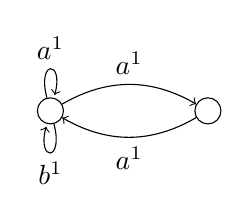
\begin{tikzpicture}
            \graphbox{}{0mm}{0mm}{32mm}{28mm}{-10mm}{-14mm}{
                \node[draw,circle] (1) at (0,0) {};
                \node[draw,circle] (2) at (2,0) {};
                \draw[->] (1) edge[loop above] node[midway, above] {$a^{1}$} (1) ;
                \draw[->] (1) edge[loop below] node[midway, below] {$b^{1}$} (1) ;
                \draw[->] (1) edge[bend left] node[midway, above] {$a^{1}$}  (2)  ;
                \draw[->] (2) edge[bend left] node[midway, below] {$a^{1}$} (1)   ;
            }
        \end{tikzpicture}
        \caption{}
        \label{fig:nwf:weighted_type_graph_grsaa_2}
    \end{figure}
     There are $t_K^{11}, t_K^{12}, t_K^{21}, t_K^{22}:K \rightarrow T$ as illustrated in~\autoref{fig:nwf:grsaa_rule_morphisms}.

    \begin{figure}[!ht]
        \centering
        \resizebox{0.49\textwidth}{!}{
            \begin{tikzpicture}
            \graphbox{\( K \)}{-50mm}{0mm}{40mm}{30mm}{2mm}{-6mm}{
                \coordinate (o) at (0mm,-10mm); 
                \node[draw,circle] (l1) at ($(o)+(-10mm,0mm)$) {1};
                \node[draw,circle] (l2) at ($(l1)+(2,0)$) {2};
                % \node[draw,circle] (l3) at ($(l1) + (1,0)$) {3};
                % \draw[] (l1) -- (l3) node[midway,above] {a};
                % \draw[] (l3) -- (l2) node[midway,above] {a};
            } 
                \graphbox{$T$}{0mm}{0mm}{40mm}{30mm}{-10mm}{-15mm}{
                    \node[draw,circle] (1) at (0,0) {$1\ 2$};
                    \node[draw,circle] (2) at (2,0) {};
                    \draw[->] (1) edge[loop above] node[midway, above] {$a$} (1) ;
                    \draw[->] (1) edge[loop below] node[midway, below] {$b$} (1) ;
                    \draw[->] (1) edge[bend left] node[midway, above] {$a$}  (2)  ;
                    \draw[->] (2) edge[bend left] node[midway, below] {$a$} (1)   ;
                }
                \node () at (-5mm,-15mm) {$\overset{t_K^{11}}{\to}$};
            \end{tikzpicture}
            } 
            \resizebox{0.49\textwidth}{!}{
            \begin{tikzpicture}
                \graphbox{\( K \)}{-50mm}{0mm}{40mm}{30mm}{2mm}{-6mm}{
                \coordinate (o) at (0mm,-10mm); 
                \node[draw,circle] (l1) at ($(o)+(-10mm,0mm)$) {1};
                \node[draw,circle] (l2) at ($(l1)+(2,0)$) {2};
                % \node[draw,circle] (l3) at ($(l1) + (1,0)$) {3};
                % \draw[] (l1) -- (l3) node[midway,above] {a};
                % \draw[] (l3) -- (l2) node[midway,above] {a};
            } 
                \graphbox{$T$}{0mm}{0mm}{40mm}{30mm}{-10mm}{-15mm}{
                    \node[draw,circle] (1) at (0,0) {$1$};
                    \node[draw,circle] (2) at (2,0) {2};
                    \draw[->] (1) edge[loop above] node[midway, above] {$a$} (1) ;
                    \draw[->] (1) edge[loop below] node[midway, below] {$b$} (1) ;
                    \draw[->] (1) edge[bend left] node[midway, above] {$a$}  (2)  ;
                    \draw[->] (2) edge[bend left] node[midway, below] {$a$} (1)   ;
                }
                \node () at (-5mm,-15mm) {$\overset{t_K^{12}}{\to}$};
            \end{tikzpicture}
            }
            \hspace{5mm}
            
            \resizebox{0.49\textwidth}{!}{
            \begin{tikzpicture}
                \graphbox{\( K \)}{-50mm}{0mm}{40mm}{30mm}{2mm}{-6mm}{
                \coordinate (o) at (0mm,-10mm); 
                \node[draw,circle] (l1) at ($(o)+(-10mm,0mm)$) {1};
                \node[draw,circle] (l2) at ($(l1)+(2,0)$) {2};
                % \node[draw,circle] (l3) at ($(l1) + (1,0)$) {3};
                % \draw[] (l1) -- (l3) node[midway,above] {a};
                % \draw[] (l3) -- (l2) node[midway,above] {a};
            } 
                \graphbox{$T$}{0mm}{0mm}{40mm}{30mm}{-10mm}{-15mm}{
                    \node[draw,circle] (1) at (0,0) {2};
                    \node[draw,circle] (2) at (2,0) {1};
                    \draw[->] (1) edge[loop above] node[midway, above] {$a$} (1) ;
                    \draw[->] (1) edge[loop below] node[midway, below] {$b$} (1) ;
                    \draw[->] (1) edge[bend left] node[midway, above] {$a$}  (2)  ;
                    \draw[->] (2) edge[bend left] node[midway, below] {$a$} (1)   ;
                }
                \node () at (-5mm,-15mm) {$\overset{t_K^{21}}{\to}$};
            \end{tikzpicture}
            }
            \resizebox{0.49\textwidth}{!}{
            \begin{tikzpicture}
                \graphbox{\( K \)}{-50mm}{0mm}{40mm}{30mm}{2mm}{-6mm}{
                \coordinate (o) at (0mm,-10mm); 
                \node[draw,circle] (l1) at ($(o)+(-10mm,0mm)$) {1};
                \node[draw,circle] (l2) at ($(l1)+(2,0)$) {2};
                % \node[draw,circle] (l3) at ($(l1) + (1,0)$) {3};
                % \draw[] (l1) -- (l3) node[midway,above] {a};
                % \draw[] (l3) -- (l2) node[midway,above] {a};
            } 
                \graphbox{$T$}{0mm}{0mm}{40mm}{30mm}{-10mm}{-15mm}{
                    \node[draw,circle] (1) at (0,0) {};
                    \node[draw,circle] (2) at (2,0) {$1\ 2$};
                    \draw[->] (1) edge[loop above] node[midway, above] {$a$} (1) ;
                    \draw[->] (1) edge[loop below] node[midway, below] {$b$} (1) ;
                    \draw[->] (1) edge[bend left] node[midway, above] {$a$}  (2)  ;
                    \draw[->] (2) edge[bend left] node[midway, below] {$a$} (1)   ;
                }
                \node () at (-5mm,-15mm) {$\overset{t_K^{22}}{\to}$};
            \end{tikzpicture}
            }
        \caption{}
        \label{fig:nwf:grsaa_rule_morphisms}
      \end{figure}
    The set $\{l \star - = t_K^{11}\}$ has two morphisms $h_{11}^1$ and $h_{11}^2$ as illustrated in~\autoref{fig:nwf:grsaa_rule_morphisms_22}.
    \begin{figure}[!ht]
        \resizebox{0.49\textwidth}{!}{
        \begin{tikzpicture}
          \graphbox{\( L \)}{-50mm}{0mm}{40mm}{40mm}{2mm}{-6mm}{
            \coordinate (o) at (0mm,-10mm); 
            \node[draw,circle] (l1) at ($(o)+(-10mm,0mm)$) {1};
            \node[draw,circle] (l2) at ($(l1)+(2,0)$) {2};
            \node[draw,circle] (l3) at ($(l1) + (1,0)$) {3};
            \draw[] (l1) -- (l3) node[midway,above] {a};
            \draw[] (l3) -- (l2) node[midway,above] {a};
        } 
            \graphbox{$T$}{0mm}{0mm}{40mm}{40mm}{-10mm}{-17mm}{
                \node[draw,circle] (1) at (0,0) {$1\ 2$};
                \node[draw,circle] (2) at (2,0) {3};
                \draw[->] (1) edge[loop above] node[midway, above] {$a^{1}$} (1) ;
                \draw[->] (1) edge[loop below] node[midway, below] {$b^{1}$} (1) ;
                \draw[->] (1) edge[bend left] node[midway, above] {$a^{1}$}  (2)  ;
                \draw[->] (2) edge[bend left] node[midway, below] {$a^{1}$} (1)   ;
            }
            \node () at (-5mm,-15mm) {$\overset{h_{11}^1}{\to}$};
        \end{tikzpicture}
        }
        \resizebox{0.49\textwidth}{!}{
            \begin{tikzpicture}
              \graphbox{\(L\)}{-50mm}{0mm}{40mm}{40mm}{2mm}{-10mm}{
                \coordinate (o) at (0mm,-10mm); 
                \node[draw,circle] (l1) at ($(o)+(-10mm,0mm)$) {1};
                \node[draw,circle] (l2) at ($(l1)+(2,0)$) {2};
                \node[draw,circle] (l3) at ($(l1) + (1,0)$) {3};
                \draw[] (l1) -- (l3) node[midway,above] {a};
                \draw[] (l3) -- (l2) node[midway,above] {a};
            } 
                \graphbox{$T$}{0mm}{0mm}{40mm}{40mm}{-10mm}{-20mm}{
                    \node[draw,circle] (1) at (0,0) {$1\ 2\ 3$};
                    \node[draw,circle] (2) at (2,0) {};
                    \draw[->] (1) edge[loop above] node[midway, above] {$a^{1}$} (1) ;
                    \draw[->] (1) edge[loop below] node[midway, below] {$b^{1}$} (1) ;
                    \draw[->] (1) edge[bend left] node[midway, above] {$a^{1}$}  (2)  ;
                    \draw[->] (2) edge[bend left] node[midway, below] {$a^{1}$} (1)   ;(1)   ;
                }
                \node () at (-5mm,-15mm) {$\overset{h_{11}^2}{\to}$};
            \end{tikzpicture}
            }
        \caption{}
        \label{fig:nwf:grsaa_rule_morphisms_22}
      \end{figure}
    Therefore, we have \begin{flalign*}
        w_\mathcal{T}(\{l \star - = t_K^{11}\})
        =&w_\mathcal{T}(\{h_{11}^1, h_{11}^2\})\\
        \overset{\mathrm{def}}{=}&w_\mathcal{T}(h_{11}^1) + w_\mathcal{T}(h_{11}^2) \\
        =&(1^1 * 1^1) + (1^1 * 1^1)\\
        =&2
    \end{flalign*}
    The set $\{r \star - = t_K^{11}\}$ has one morphism $h_{11}^3$ as illustrated in~\autoref{wf:example:context_closure_grs_aa}.
    \begin{figure}[!ht]
        \centering
        \resizebox{0.49\textwidth}{!}{
        \begin{tikzpicture}
          \graphbox{\( R \)}{-55mm}{0mm}{45mm}{44mm}{1mm}{-22mm}{
            \coordinate (o) at (-5mm,-3mm); 
            \node[draw,circle] (l1) at ($(o)+(-10mm,0mm)$) {1};
            \node[draw,circle] (l2) at ($(l1)+(3,0)$) {2};
            \node[draw,circle] (l3) at ($(l1) + (1,0)$) {4};
            \node[draw,circle] (l4) at ($(l1) + (2,0)$) {5};
            \draw[->] (l1) -- (l3) node[midway,above] {a};
            \draw[->] (l3) -- (l4) node[midway,above] {b};
            \draw[->] (l4) -- (l2) node[midway,above] {a};
        } 
            \graphbox{$T$}{0mm}{0mm}{40mm}{44mm}{-10mm}{-22mm}{
                \node[draw,circle] (1) at (0,0) {$1\ 2\ 4\ 5$};
                \node[draw,circle] (2) at (2,0) {};
                \draw[->] (1) edge[loop above] node[midway, above] {$a^{1}$} (1) ;
                \draw[->] (1) edge[loop below] node[midway, below] {$b^{1}$} (1) ;
                \draw[->] (1) edge[bend left] node[midway, above] {$a^{1}$}  (2)  ;
                \draw[->] (2) edge[bend left] node[midway, below] {$a^{1}$} (1)   ;
            }
            \node () at (-5mm,-19mm) {$\overset{h_{11}^3}{\to}$};
        \end{tikzpicture}
        }
        \caption{}
        \label{wf:example:context_closure_grs_aa}
      \end{figure}
    Therefore, we have: $w_\mathcal{T}(\{r \star - = t_K^{11}\}) = w_\mathcal{T}(h_{11}^3) = 1^1 * 1^1 * 1 ^ 1 = 1$. Thus, we have $w_\mathcal{T}(\{l \star - = t_K^{11}\}) = 2 \geq 1 = w_\mathcal{T}(\{r \star - = t_K^{11}\})$.

    Similarly, we can check that $w_\mathcal{T}(\{l \star - = t_K^{12}\}) = 1 \geq 1 = w_\mathcal{T}(\{r \star - = t_K^{12}\})$,  $w_\mathcal{T}(\{l \star - = t_K^{21}\}) = 1 \geq 1 = w_\mathcal{T}(\{r \star - = t_K^{21}\})$, and $w_\mathcal{T}(\{l \star - = t_K^{22}\}) = 1 \geq 1 = w_\mathcal{T}(\{r \star - = t_K^{22}\})$. The rule is therefore weakly decreasing.

    There exists a context closure $c$ for the DPO rule in the weighted type graph, as shown in \autoref{wf:example:context_closure}.
    Since we have additionally $t_K^{11} = l \star c$ and $w_\mathcal{T}(\{l \star - = t_K^{11}\}) = 2 > 1 = w_\mathcal{T}(\{r \star - = t_K^{11}\})$, the rule is closure decreasing since the semiring is strictly monotonic.
\end{example} 
 
\subsection{Termination Criterion}
\label{wf:sec:termination}
\begin{theorem}[Termination of DPO rewriting system~\cite{endrullis2024generalized_icgt}] 
    \label{wf:thm:termination_grs}
    Let $\mathcal{A}$ and $\mathcal{B}$ be sets of DPO rewriting rules, $\mathcal{T} = (T,\mathbb{E}, (S, \oplus, \odot, 0_S, 1_S, \prec, \leq), w)$ a finitary weighted type graph and $\mathfrak{F}$ a DPO rewriting framework such that

        \begin{itemize}
            \item \(\operatorname{left}(\Delta)\) is weighable with \(\mathcal{T}\),
            \item \(\operatorname{right}(\Delta)\) is bounded above by \(\mathcal{T}\). 
        \end{itemize}
    for every rule $\rho \in (\mathcal{A }\cup \mathcal{B })$ and every double pushout diagram  
        $\Delta \in \mathfrak{F}(\rho)$. If the following conditions hold:
    \begin{enumerate}
        \item either every $\rho \in \mathcal{A}$ is uniformly decreasing or every $\rho \in \mathcal{A}$ is closure decreasing, and
        \item every rule $\rho \in \mathcal{B}$ is weakly decreasing,
    \end{enumerate}
    then $\Rightarrow_{\mathcal{A},\mathfrak{F}}$ is \textbf{terminating} relative to $\Rightarrow_{\mathcal{B},\mathfrak{F}}$.
\end{theorem} 
\begin{example} 
    \label{wf:example:termination}
    Termination of the DPO rule in \autoref{ex:grsaa} can be established using \autoref{wf:thm:termination_grs} together with the weighted type graph in \autoref{wf:example:weighted_type_graph} over the natural arithmetic semiring $\mathfrak{N} = (\mathbb{N},+,*,0_\mathbb{R},1_\mathbb{N},<,\leq)$. It is closure decreasing by \autoref{wf:example:decreasing_rule}.
\end{example}
